\documentclass[a4paper,10pt,abstracton]{scrartcl}

\usepackage[margin=2.5cm]{geometry}
\usepackage{graphicx}
\usepackage[UKenglish]{babel}
\usepackage{csquotes}
\usepackage[style=numeric,citestyle=numeric,backend=biber,sorting=none,doi=false,url=false]{biblatex}
\usepackage{float}
\usepackage[export]{adjustbox}
\usepackage[T1]{fontenc}
\usepackage{lmodern}
\usepackage{todonotes}
\usepackage[labelsep=period,font=small,labelfont=bf,format=plain]{caption}
\usepackage[group-separator={,}]{siunitx}
\usepackage{booktabs}

\title{The evolution and spread of target-site resistance to DDT and pyrethroids in the malaria vectors \emph{Anopheles gambiae} and \emph{Anopheles coluzzii}}

\subtitle{DRAFT}

\author{
	Chris S. Clarkson
	\and 
	Alistair Miles
	\and
	Nicholas J. Harding
        \and
        ...
	\and
	Dominic Kwiatkowski
	\and
	Martin Donnelly
	\and
	The Anopheles gambiae 1000 Genomes Consortium
} 
%\date{January 21, 1994}

\begin{document}

\maketitle

\begin{abstract}

%%
TODO

\end{abstract}

\section*{Introduction}

The malaria vectors \emph{Anopheles gambiae} and \emph{Anopheles
  coluzzii} are evolving insecticide resistance asdlkj dsalkj daslkjd
aslkjdas lkadsj lkadsj adslkj adslkja dslkadsj lkadsj lkasd jlkads
jlkadsj lkads jlakds alksdj asdlk jasdlk adslk jadslkj adslkj adslkj
adslkj adslkj adslk jasd

This is the second paragraph of the introduction, asdlkjio weipo
ewrpoi ewrpoi rwepoi werpoiwre poi rewpoi rwepoi erwpoi rewpoi rwepoi
rwepoi rwepoi rewpo iwrepoi rwepoi wrepoi wrepoi rwpeo irwpo irwepoi
rwepo ipoewi rpow ierwe

Third paragraph zcx,m ncxz,mxczn ,mxczn,mxcz n,mcnxz ,mxczn ,mz ncx,m
zcxn

Fourth paragraph asdlkj dsakljdsalkj dsalkj daslkj daslkj dsalkj
daslkj sda

TODO

\section*{Results}

Let's add some results qweoi qewoiewqoip peqwpoi ewqpoi ewqpoieqwipo
ewqipo eqwpio eqwipo ewqoip ewqoip ewqiop eqw

Isn't Figure \ref{fig:demo} interesting! Table \ref{table:demo} is
pretty interesting too.

\begin{figure}[t!]
  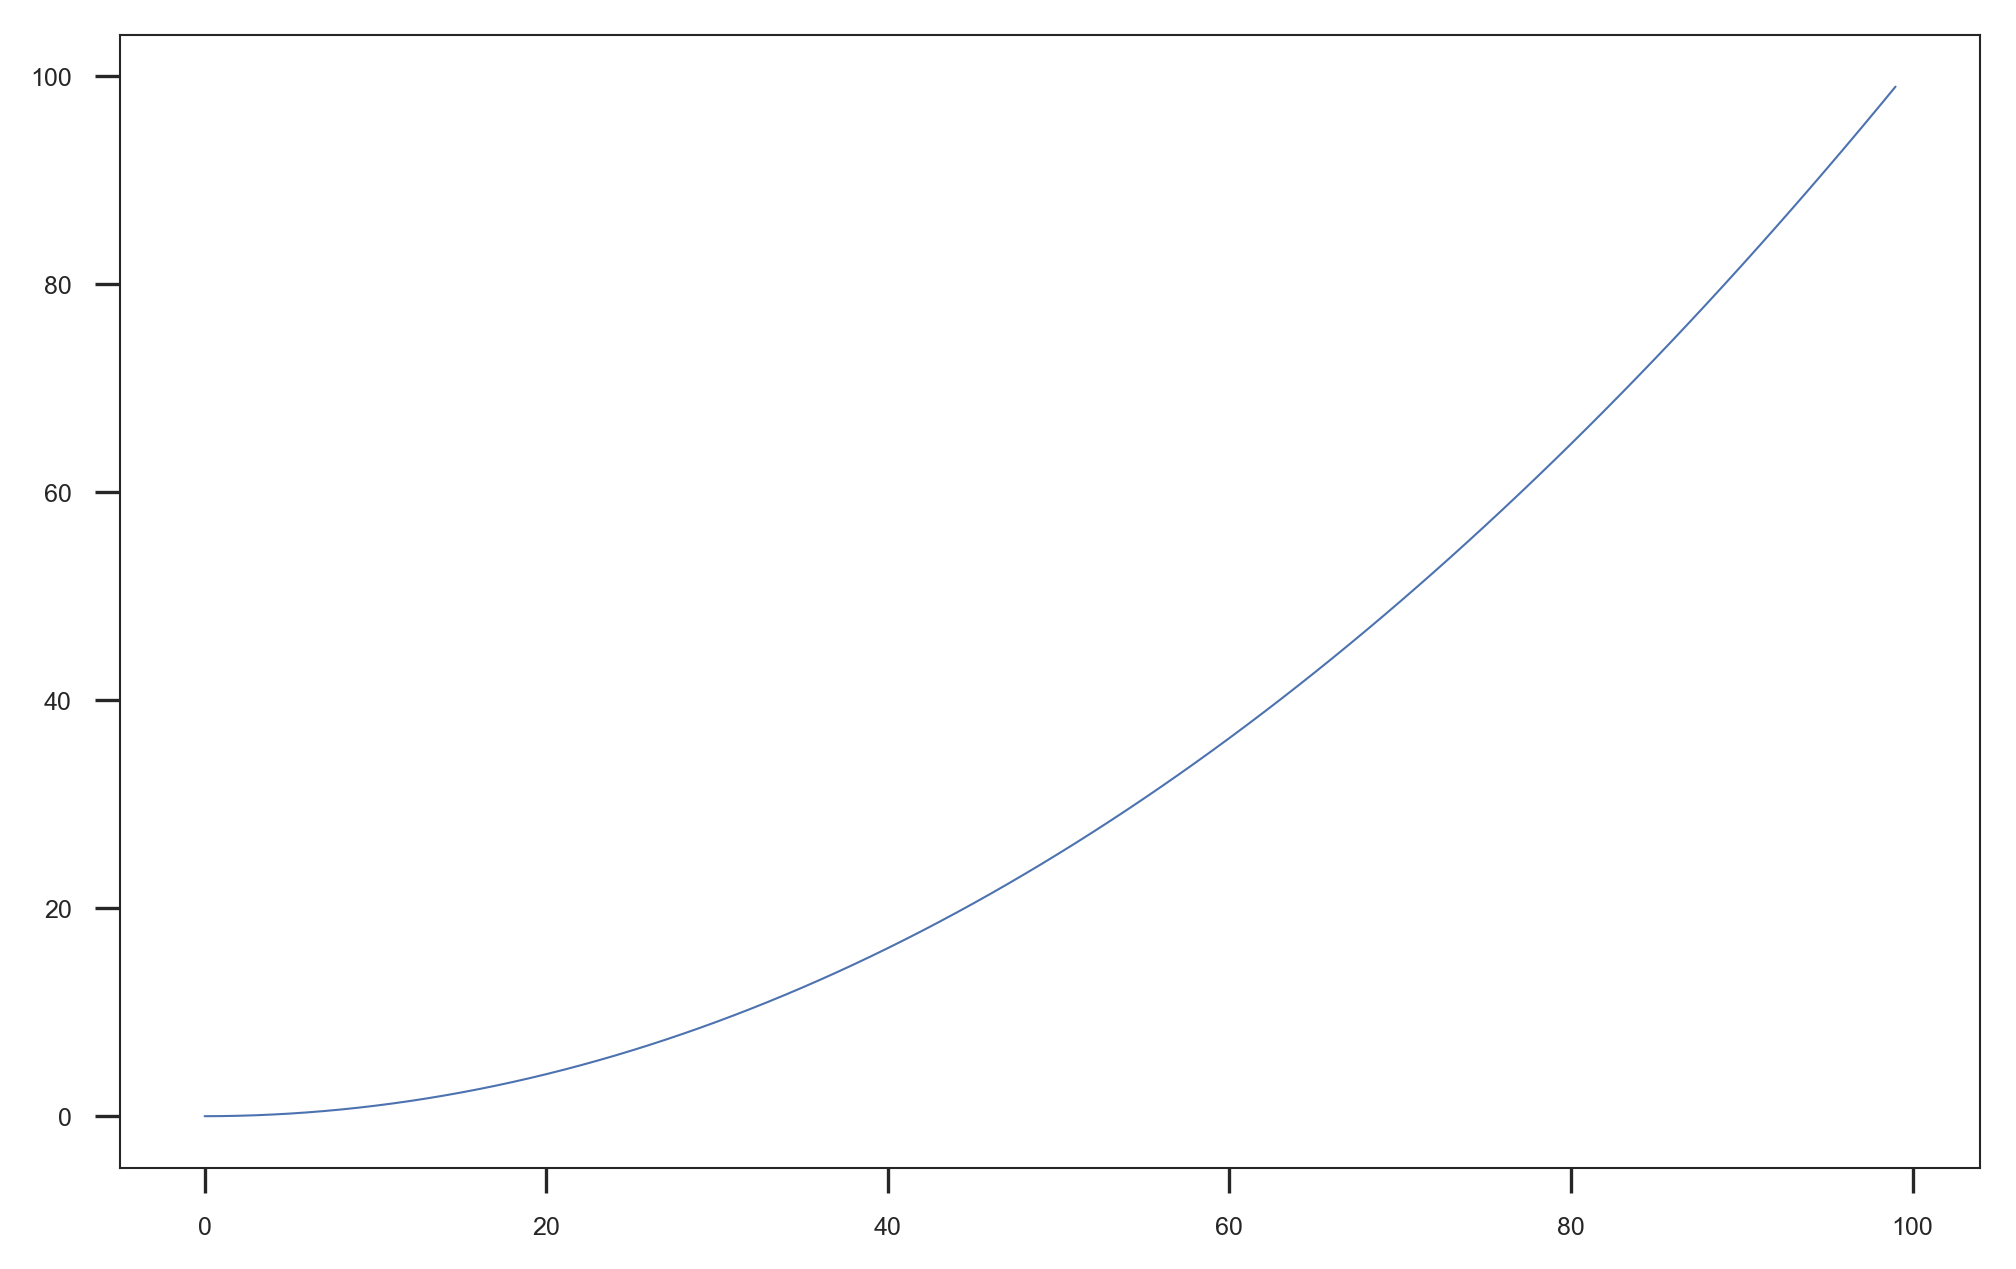
\includegraphics[width=1.1\linewidth,center]{artwork/demo.png}
  \caption{Demo figure.}
  \label{fig:demo}
\end{figure}

TODO

\begin{table}[h]
  \centering
  
\begin{tabular}{rll}
\toprule
Foo & Bar & Baz \\
\midrule

1 & a & True \\

2 & b & False \\

\bottomrule
\end{tabular}

  \caption{This is a table.}
  \label{table:demo}
\end{table}

\section*{Discussion}

TODO

\section*{Methods}

TODO

\end{document}
